\documentclass{beamer}
\usetheme{Madrid}
\usecolortheme{dolphin}
\usepackage{graphicx}
\usepackage{amsmath}
\usepackage{tikz}
\usetikzlibrary{arrows.meta, positioning}
\usepackage{hyperref}
\usepackage{comment}

\title{Medical Prescription Recognition for Efficient Healthcare Workflows}
\author{Nabeel Ahmed \\ M240464CS}
\institute{Guided by: Sumesh TA}
\date{May 2026}

\begin{document}

\begin{frame}
\titlepage
\end{frame}

\begin{frame}{Outline}
\tableofcontents
\end{frame}

\section{Introduction}

\begin{frame}{Introduction}
\begin{itemize}
    \item \textbf{Medication errors} from illegible prescriptions are a critical healthcare challenge
    \item WHO estimates that 1 death per million population occurs annually ($\approx$ 163,000 deaths in EU)~\cite{bhuiyan2022online}
    \item \textbf{97.1\%} of doctors in developing countries still use handwritten prescriptions~\cite{bhuiyan2022online}
    \item \textbf{Key challenges:}
    \begin{itemize}
        \item Mixed content documents (printed + handwritten)~\cite{fang2023improved}
        \item Specialized medical terminology~\cite{lee2020biobert}
        \item Multilingual requirements~\cite{pavithiran2024multilingual}
        \item Time-critical processing needs~\cite{irjmets2024}
    \end{itemize}
\end{itemize}
\end{frame}

\begin{frame}{Problem Statement}
Handwritten medical prescriptions are difficult to digitize due to inconsistent handwriting, mixed printed and handwritten regions, and frequent image quality issues. These challenges make it hard to accurately extract medication details and can lead to serious dispensing errors, as highlighted by Bhuiyan et al. \cite{bhuiyan2022online}. This project aims to develop a reliable end-to-end system that can segment prescription regions, recognize handwritten text, and validate extracted information to support safer and more efficient healthcare workflows.
\end{frame}

\section{Literature Review}

\begin{frame}{Literature Review: Contd..}
\textbf{Tabassum et al. (2022), Nature Scientific Reports~\cite{tabassum2021recognition}}
\begin{itemize}
    \item Created 'Handwritten Medical Term Corpus' with 17,431 samples
    \item Introduced RSS (Rotate-Shift-Stretch) data augmentation
    \begin{itemize}
        \item Expanded dataset to 1,591,100 samples
        \item Represents real-world handwriting diversity
    \end{itemize}
    \item Bidirectional LSTM architecture
    \item 93.0\% average accuracy (94.5\% max)
    \item 19.6\% improvement over non-augmented approaches
\end{itemize}
\end{frame}

\begin{frame}{Literature Review Contd..}
\textbf{Pavithiran et al. (2024)~\cite{pavithiran2024multilingual}}
\begin{itemize}
    \item Hybrid CNN-RNN-LSTM architecture
    \item Unicode support for multilingual prescriptions
    \item 89\% accuracy on multi-language datasets
\end{itemize}


\textbf{Utkarsh Shaw et al., 2021)~\cite{utkarshaw2021}}
  \begin{itemize}
  \item Three-layer neural network using EMNIST dataset
  \item 94.49\% training accuracy, 80.72\% test accuracy
  \item Segmentation of handwritten strokes into individual characters
  \end{itemize}
\end{frame}

\begin{frame}{Literature Review Contd..}
\textbf{Dhar et al. (2020), Springer Multimedia Tools and Applications~\cite{dhar2020method}}
\begin{itemize}
    \item Novel method for separating printed and handwritten text in prescriptions
    \item Uses gradient-based features and ensemble classifiers
    \item Addresses critical preprocessing challenge for prescription analysis
    \item Achieved 97.8\% classification accuracy on mixed-content documents
\end{itemize}

\textbf{Fajardo et al. (2019), IEEE HNICEM~\cite{fajardo2019doctor}}
\begin{itemize}
    \item Deep learning approach for cursive handwriting in medical contexts
    \item Custom CNN architecture optimized for doctor's handwriting patterns
    \item Demonstrated effectiveness on Philippine prescription dataset
    \item Incorporated specialized preprocessing for varying ink intensities
\end{itemize}
\end{frame}

\section{Proposed Methodology}

\begin{frame}{System Architecture}
\begin{center}
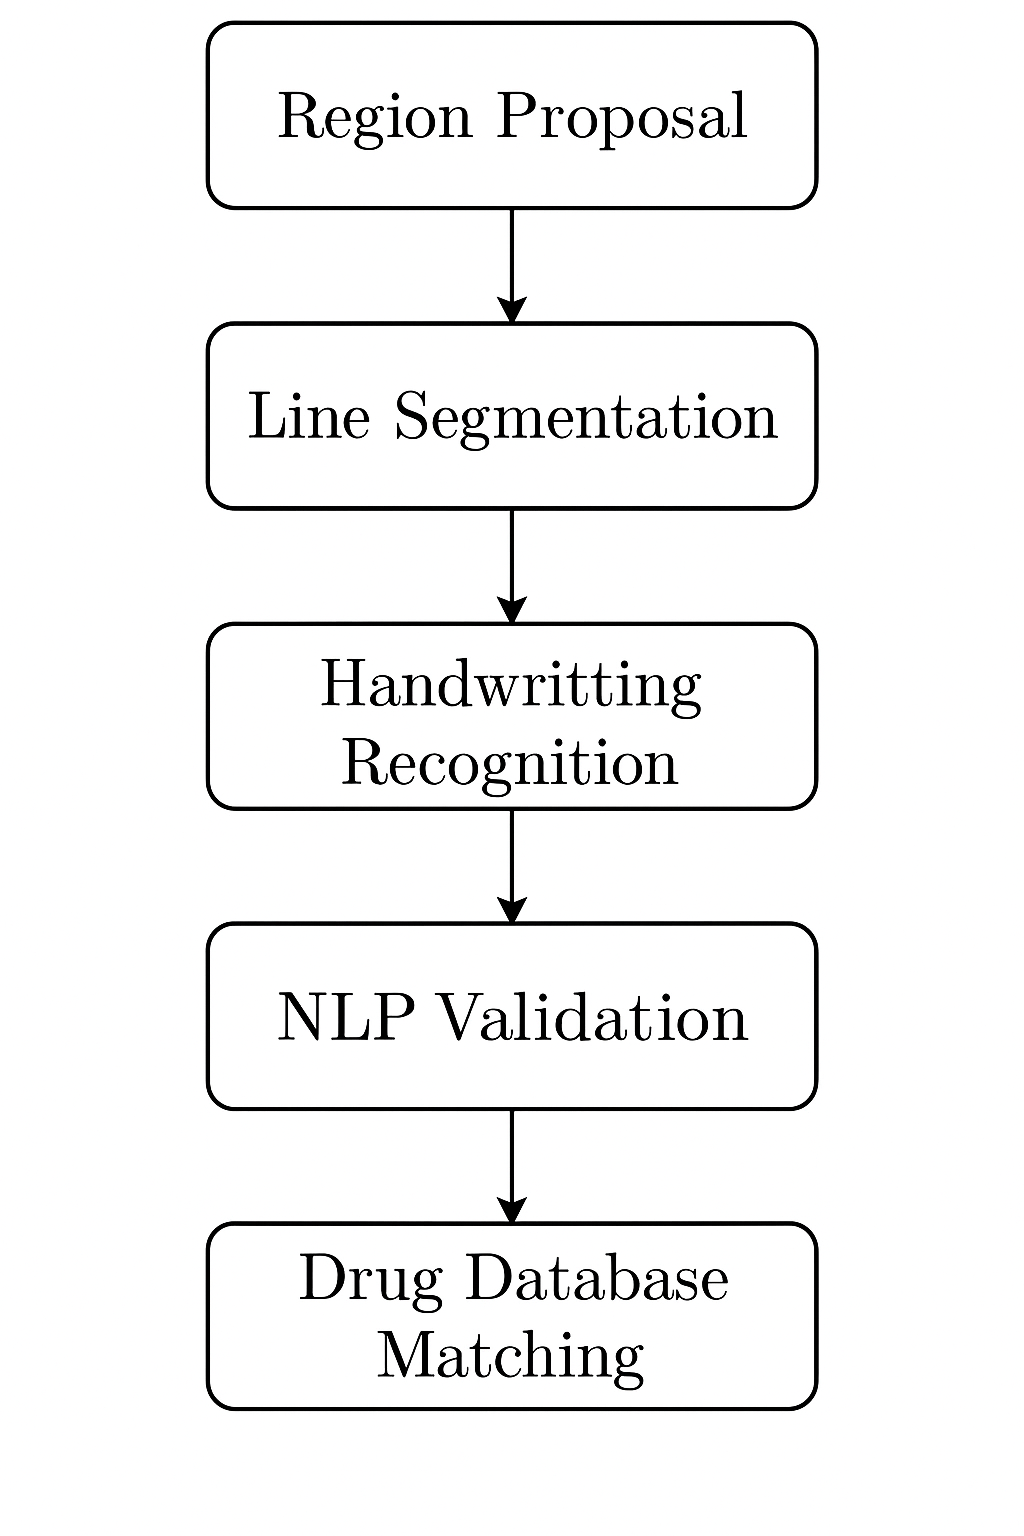
\includegraphics[height=0.7\textwidth]{archetecture phase2}
\end{center}
\end{frame}

\begin{frame}{System Overview}
\textbf{Implemented region-aware pipeline:}
\begin{enumerate}
    \item Preprocessing: illumination compensation, thresholding, normalization
    \item Handwritten-region detection using YOLO bounding boxes
    \item OpenCV line and word segmentation
    \item Word-level TrOCR medicine-name recognition~\cite{mishra2022trocr}
    \item Dosage/frequency rules + drug lexicon matching
\end{enumerate}

\vspace{0.25cm}
\centering
\resizebox{\textwidth}{!}{
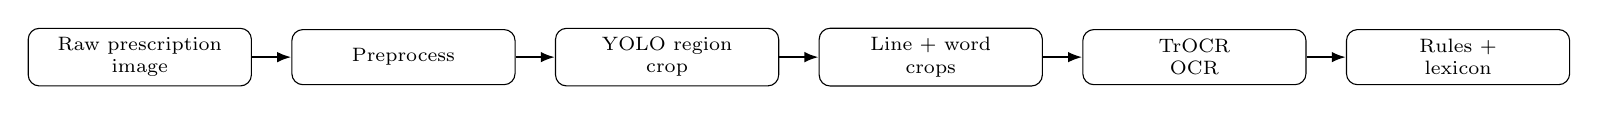
\begin{tikzpicture}[
  node distance=5mm,
  block/.style={draw, rounded corners, align=center, minimum height=7mm, text width=2.6cm, font=\scriptsize},
  arrow/.style={-{Latex[length=1.8mm]}, thick}
]
\node[block] (raw) {Raw prescription\\image};
\node[block, right=of raw] (pre) {Preprocess};
\node[block, right=of pre] (reg) {YOLO region\\crop};
\node[block, right=of reg] (seg) {Line + word\\crops};
\node[block, right=of seg] (ocr) {TrOCR\\OCR};
\node[block, right=of ocr] (val) {Rules +\\lexicon};
\draw[arrow] (raw) -- (pre);
\draw[arrow] (pre) -- (reg);
\draw[arrow] (reg) -- (seg);
\draw[arrow] (seg) -- (ocr);
\draw[arrow] (ocr) -- (val);
\end{tikzpicture}}
\end{frame}

\begin{frame}{Data Acquisition and Preparation}
\textbf{Datasets:}
\begin{itemize}
    \item Doctor's Handwritten Prescription BD cropped-word dataset
    \item Two additional cropped medicine-word datasets
    \item \textbf{Combined TrOCR dataset:} 8274 train, 1033 validation, 1040 test samples before augmentation
    \item Custom full-prescription images used for region/line/word annotation workflow
\end{itemize}

\textbf{Train-time augmentation:}
\begin{itemize}
    \item Rotation, translation, scaling
    \item Contrast variation, blur, noise
    \item Applied only to training split to avoid validation/test leakage
\end{itemize}
\end{frame}

\begin{frame}{Region Detection Module}
\textbf{YOLO handwritten-region detector:}
\begin{itemize}
    \item Detects the prescription handwritten region as a bounding box
    \item Replaces fragile heuristic cropper
    \item Labels come from corrected manual/CVAT-style region boxes
    \item Stable model copied to \texttt{models/region\_yolo\_best.pt}
\end{itemize}

\vspace{0.1cm}
\textbf{Latest validation on small split:}
\begin{itemize}
    \item Precision: 99.40\%, Recall: 100.00\%
    \item mAP@0.5: 99.50\%, mAP@0.5:0.95: 92.90\%
\end{itemize}

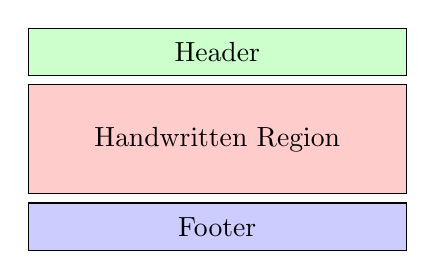
\begin{tikzpicture}[scale=0.6]
\draw[fill=blue!20] (0,0) rectangle (8,1) node[pos=.5] {Footer};
\draw[fill=red!20] (0,1.2) rectangle (8,3.5) node[pos=.5] {Handwritten Region};
\draw[fill=green!20] (0,3.7) rectangle (8,4.7) node[pos=.5] {Header};
\end{tikzpicture}
\end{frame}

\begin{frame}{Handwriting Recognition Pipeline}
\textbf{TrOCR medicine-word OCR:}
\begin{itemize}
    \item Base model: \texttt{microsoft/trocr-base-handwritten}
    \item Fine-tuned on combined cropped medicine-word dataset
    \item Final OCR unit is a word crop, not the whole page
    \item Beam-search decoding and text normalization during evaluation
\end{itemize}

\textbf{Workflow:}
\begin{enumerate}
    \item Detect handwritten region
    \item Segment line crops and word crops
    \item Feed word crop to TrOCR
    \item Validate medicine prediction using rules and lexicon
\end{enumerate}
\end{frame}

\begin{frame}{What We Added Around TrOCR}
\centering
\resizebox{0.92\textwidth}{!}{
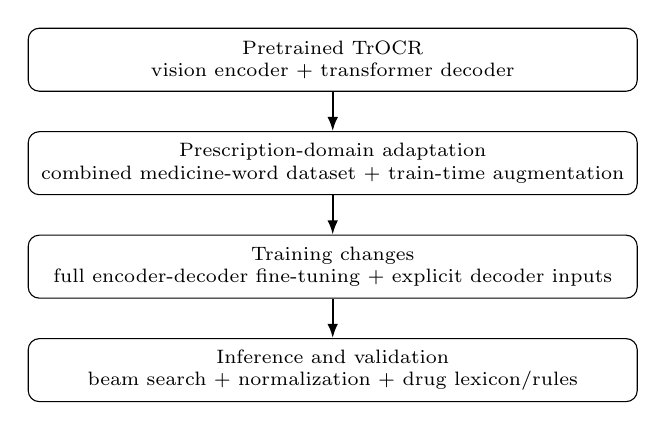
\begin{tikzpicture}[
  node distance=5mm,
  block/.style={draw, rounded corners, align=center, minimum height=8mm, text width=7.5cm, font=\scriptsize},
  arrow/.style={-{Latex[length=1.8mm]}, thick}
]
\node[block] (base) {Pretrained TrOCR\\vision encoder + transformer decoder};
\node[block, below=of base] (data) {Prescription-domain adaptation\\combined medicine-word dataset + train-time augmentation};
\node[block, below=of data] (train) {Training changes\\full encoder-decoder fine-tuning + explicit decoder inputs};
\node[block, below=of train] (decode) {Inference and validation\\beam search + normalization + drug lexicon/rules};
\draw[arrow] (base) -- (data);
\draw[arrow] (data) -- (train);
\draw[arrow] (train) -- (decode);
\end{tikzpicture}}

\vspace{0.25cm}
\small
\textbf{Novelty is domain adaptation and pipeline integration, not a new transformer architecture.}
\end{frame}

\begin{frame}{Validation Module}
\textbf{Drug lexicon matching:}
\begin{itemize}
    \item Fuzzy similarity to correct small OCR mistakes
    \item Flags uncertain medicine-name predictions for review
\end{itemize}

\textbf{Dosage/frequency extraction:}
\begin{itemize}
    \item Regex rules for expressions such as \texttt{500 mg}, \texttt{BD}, \texttt{1-0-1}
    \item BioBERT NER is kept as a future extension, not used in current metrics
\end{itemize}
\end{frame}
\begin{frame}{Experimental Results}

\begin{columns}

% ---------- LEFT COLUMN ----------
\begin{column}{0.48\textwidth}
\textbf{Recognition Output:}


\vspace{0.35cm}
\begin{figure}
    \centering
    % Replace "sample_output.png" with your uploaded image
    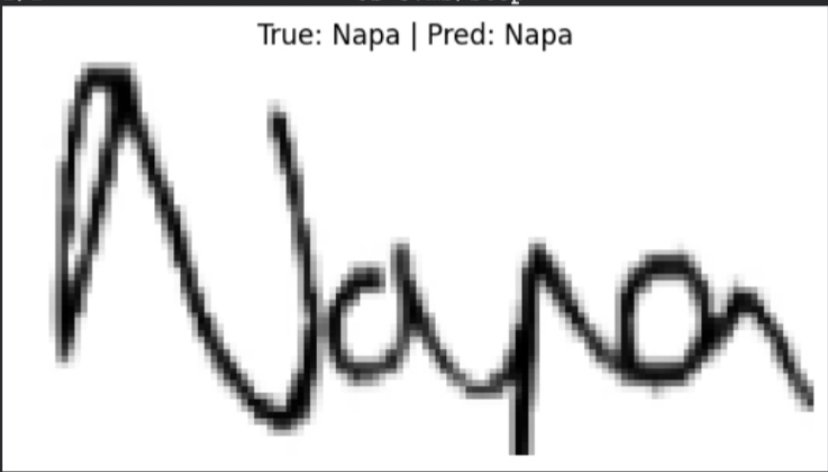
\includegraphics[width=\linewidth]{output2.png}
   
\end{figure}

\end{column}

% ---------- RIGHT COLUMN ----------
\begin{column}{0.48\textwidth}


\vspace{0.35cm}
\begin{figure}
    \centering
    % Replace "metrics_graph.png" with your graph image
    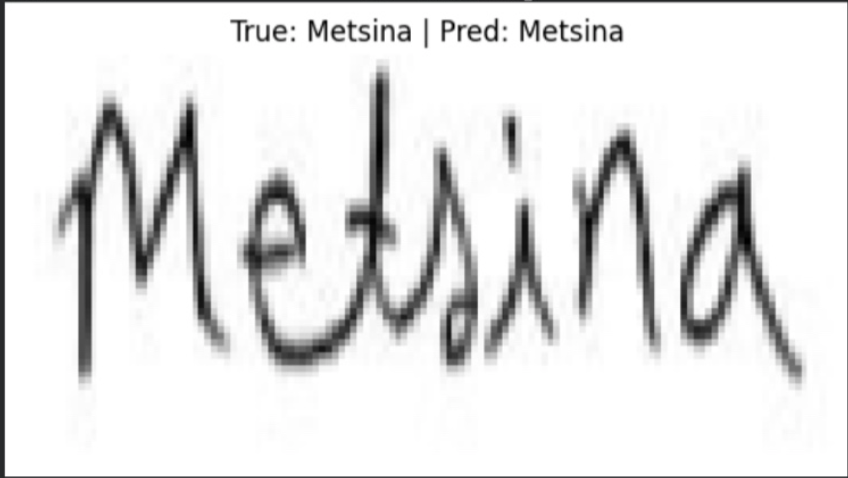
\includegraphics[width=\linewidth]{output1.png}

\end{figure}
\begin{figure}
    \centering
    % Replace "metrics_graph.png" with your graph image
    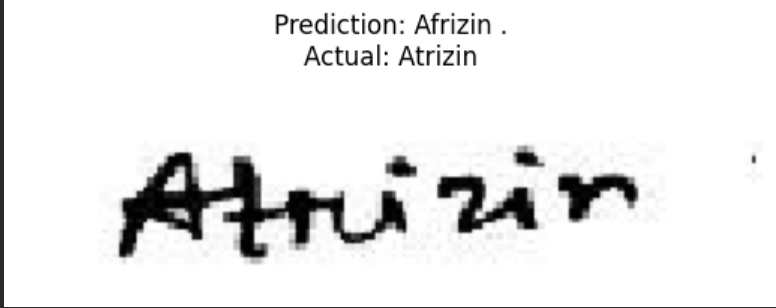
\includegraphics[width=\linewidth]{output3.png}

\end{figure}

\vspace{0.25cm}



\end{column}

\end{columns}

\end{frame}

\begin{frame}{Evaluation Metrics}

\centering
\textbf{Phase 4 OCR Module (Medicine Name Recognition)} \\
\vspace{0.4cm}

\small
Model: \texttt{microsoft/trocr-base-handwritten} (fine-tuned) \\
Dataset: Combined cropped-word dataset (Validation split, $n=1033$) \\
\normalsize

\begin{table}[h!]
\centering
\renewcommand{\arraystretch}{1.3} % row spacing
\begin{tabular}{l c}
\hline
\textbf{Metric} & \textbf{Value} \\
\hline
Strict Exact-Match Accuracy & 83.16\% \\
Case-Insensitive Exact-Match & 89.06\% \\
Character Error Rate (CER) & 5.91\% \\
Word Error Rate (WER) & 17.02\% \\
Validation Loss & 0.2076 \\
Training Steps & 2500 \\
\hline
\end{tabular}
\end{table}

\end{frame}

\begin{frame}{Small GPT/LLM OCR Comparison}
\small
\textbf{Manual GPT/LLM recognition sample:} 12 cropped medicine-word examples.\\
\textit{This is an illustrative comparison only; it is not the same-sized validation split used for TrOCR.}

\vspace{0.25cm}
\begin{columns}
\begin{column}{0.48\textwidth}
\centering
\renewcommand{\arraystretch}{1.2}
\begin{tabular}{l c}
\hline
\textbf{Metric} & \textbf{GPT/LLM} \\
\hline
Strict exact match & 50.00\% \\
Case-insensitive exact & 58.33\% \\
CER & 30.00\% \\
WER & 53.85\% \\
Samples & 12 \\
\hline
\end{tabular}
\end{column}
\begin{column}{0.48\textwidth}
\centering
\renewcommand{\arraystretch}{1.2}
\begin{tabular}{l c}
\hline
\textbf{Metric} & \textbf{Our TrOCR} \\
\hline
Strict exact match & 83.16\% \\
Case-insensitive exact & 89.06\% \\
CER & 5.91\% \\
WER & 17.02\% \\
Samples & 1033 \\
\hline
\end{tabular}
\end{column}
\end{columns}

\vspace{0.25cm}
\footnotesize
Examples of GPT/LLM errors: \texttt{nexe} $\rightarrow$ \texttt{Neel}, \texttt{Zo.mups 20} $\rightarrow$ \texttt{20-mg}, \texttt{Progut} $\rightarrow$ \texttt{Pmgt}.
\end{frame}


\section{Comparison with Prior Work}

\begin{frame}{Comparison with Similar Works}
\centering
\small
\begin{table}[h!]
\centering
\renewcommand{\arraystretch}{1.15}
\begin{tabular}{p{3.1cm} p{2.4cm} c}
\hline
\textbf{Work} & \textbf{Reported Metric} & \textbf{Value} \\
\hline
Tabassum et al. (2022) & Recognition Accuracy & 93.0\% \\
Pavithiran et al. (2024) & Recognition Accuracy & 89.0\% \\
Utkarsh Shaw et al. (2021) & Test Accuracy & 80.72\% \\
\textbf{This Work} & \textbf{Strict Exact Match} & \textbf{83.16\%} \\
\textbf{This Work} & \textbf{Case-insensitive Exact Match} & \textbf{89.06\%} \\
\hline
\end{tabular}
\end{table}

\vspace{0.2cm}
\footnotesize
\textbf{Short Comparison:}
\begin{itemize}
    \item Current result is on a larger, mixed-source dataset, so it is more realistic than the earlier single-source result.
    \item We report stricter OCR quality metrics: CER 5.91\% and WER 17.02\%.
    \item Metrics are for cropped-word OCR; full-page accuracy depends on region, line, and word segmentation quality.
\end{itemize}
\end{frame}


\begin{frame}{Work Done}
\begin{itemize}
    \item Combined three cropped-word prescription datasets for TrOCR training
    \item Added train-time augmentation for handwriting robustness
    \item Fine-tuned TrOCR (\texttt{trocr-base-handwritten}) with full encoder-decoder training
    \item Implemented preprocessing, YOLO region cropping, and OpenCV line/word segmentation
    \item Added final end-to-end runner that outputs medicine, dosage, frequency, and validation status as CSV/JSON
\end{itemize}
\end{frame}

\begin{frame}{Final Prototype Implementation}
\textbf{Implemented end-to-end flow:}
\begin{enumerate}
    \item Raw prescription image preprocessing
    \item Handwritten-region extraction using YOLO detector
    \item Line and word crop generation
    \item TrOCR inference using fine-tuned checkpoint
    \item Drug lexicon matching with dosage/frequency extraction
\end{enumerate}

\vspace{0.2cm}
\textbf{Outputs:}
\begin{itemize}
    \item Page, region, line, and word manifests
    \item Cropped images for human review
    \item Structured \texttt{predictions.csv}/\texttt{predictions.json}
\end{itemize}
\end{frame}


\begin{frame}{Novelty in Approach}
\begin{itemize}
    \item \textbf{Region-aware processing:} avoids whole-page OCR by isolating handwritten regions first.
    \item \textbf{TrOCR domain adaptation:} combined medical word data, train-time augmentation, full fine-tuning, beam search.
    \item \textbf{Training stability fix:} explicit decoder-input preparation for TrOCR training.
    \item \textbf{Reviewable pipeline:} stores manifests and crops at each stage for medical audit.
    \item \textbf{Validation layer:} combines OCR with dosage/frequency rules and drug lexicon matching.
\end{itemize}
\end{frame}




\section{Conclusion}

\begin{frame}{Conclusion}
\textbf{Current outcome:}
\begin{itemize}
    \item Region-aware pipeline implemented from page image to structured prediction.
    \item TrOCR validation: 83.16\% strict exact match, 89.06\% case-insensitive exact match.
    \item YOLO region detector gives strong preliminary region-crop results on the small validation split.
\end{itemize}

\textbf{Future Work:}
\begin{itemize}
    \item Complete final test-set evaluation from saved best TrOCR checkpoint
    \item Larger reviewed full-page dataset for end-to-end quantitative evaluation
    \item Integration with hospital electronic health record systems
    \item BioBERT-style NER and larger Indian drug lexicon
\end{itemize}

\textbf{Practical Impact:} Potential reduction in prescription interpretation errors, addressing a critical healthcare challenge that contributes to thousands of preventable adverse drug events annually~\cite{bhuiyan2022online}
\end{frame}

\begin{frame}[allowframebreaks]{References}
\bibliographystyle{abbrv}
\bibliography{references}
\end{frame}

\end{document}
